\chapter{Generalizing Pooling Functions in CNNs: Mixed, Gated, and Tree}

{\small \textbf{Authors}\\
Chen-Yu Lee, Patrick Gallagher and Zhuowen Tu\\ \\
IEEE TRANSACTIONS ON PATTERN ANALYSIS AND MACHINE INTELLIGENCE\\VOL. 40, NO. 4, APRIL 2018}

\section{Proposed Method}

The pooling layer has already been presented in the overview of this report but here we will talk about it going more in depth. The pooling operation is usually employed in CNNs because downsamples the feature maps ending up with smaller resolutions, and for this reason is quite convenient to use it because we aim at gradually reducing the size of our layers while we move through them. There are a few pooling operations but in this paper we will take into account mainly two of them: the \textit{max} and the \textit{average} pooling. In the first one we take the max over 4 numbers (if we have $2 \times 2$ regions in some depth). In the second one we take the average. It should be noted that the depth dimension remains the same. More specifically, in the following paper, we will propose two approaches to generalize pooling. The first approach is split into two strategies that are respectively: \textit{mixed max-average pooling} and \textit{gated max-average pooling}. As our main goal is to obtain a good responsiveness into our pooling functions, we will decide if these two strategies are responsive or unresponsive depending on how well they are able to generalize. Mixed max-average pooling, is said to be unresponsive because it is only a standard combination of max and average pooling and it does not react to the features of the pooled region. On the other hand, in gated max-average pooling, we notice a responsiveness to changes in the pooled region. After having pointed out this main difference, let us explain how they both are implemented. As far as the mixed max-average pooling, we have a parameter called $a$ that is defined between 0 and 1 and basically is a scalar that allows us to balance the amount of max pooling and average pooling into our general equation that is:

\begin{equation}
    \label{eq:08_1}
    f_{mix}(\textbf{x}) = a_{\ell} \cdot f_{max}(\textbf{x})+(1- a_{\ell}) \cdot f_{avg}(\textbf{x})
\end{equation}\\
In gated max-average pooling instead, we are still trying to learn a proportion but this time we use a gating mask that is multiplied with the region we mean to pool and the result is used to apply a sigmoid activation function. In Figure \ref{fig:08_1} we show an illustration of both methods.\\

\begin{equation}
    \label{eq:08_2}
    f_{gate}(\textbf{x}) = \sigma(\mathbold{\omega}^T\textbf{x})f_{max}(\textbf{x})+(1-\sigma(\mathbold{\omega}^T\textbf{x}))f_{avg}(\textbf{x})
\end{equation}

\begin{figure}[h!]
    \centering
    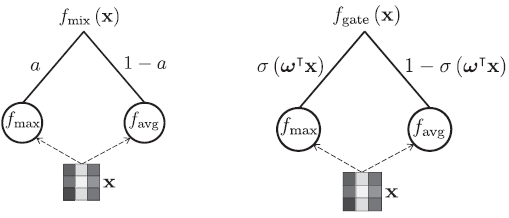
\includegraphics[scale=0.75]{images/08_1.png}
    \caption{Left: mixed max-average pooling. Right: gated max-average pooling.}
    \label{fig:08_1}
\end{figure}

\FloatBarrier

Another way to understand how to generalize pooling, is by combining its operations between them in order to learn the parameters that we need in the filters by themselves. How we can do that? We use trees. More specifically we use decision trees whose aim is to learn filters and how they can be combined. To better understand how they work we provide an illustration as shown in Figure \ref{fig:08_2}

\begin{figure}[h!]
    \centering
    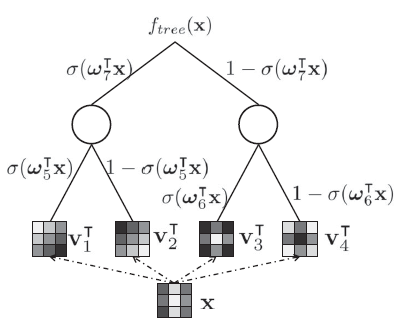
\includegraphics[scale=0.65]{images/08_2.png}
    \caption{Tree pooling operation.}
    \label{fig:08_2}
\end{figure}

\FloatBarrier

As we can see, this tree has three levels and each leaf is a filter we want to learn. If we have only one node we end up with only $\textbf{v}_m^T \textbf{x}$. Instead, if we have more nodes, we combine the result of both left and right children with the strategy presented in gated max-average pooling.

\section{Experimental Results}

Experiments have been conducted on five datasets. They are MNIST \citep{MNIST}, CIFAR10 \citep{CIFAR10and100}, CIFAR100 \citep{CIFAR10and100}, SVHN \citep{SVHN} and ImageNet \citep{ImageNet12}. It turns out that by applying the proposed methods we must sacrifice the time execution by a range of 5-15\%. But it has been proved that it is not a big issue as it is quite easy to implement and it is worth it. In order to achieve better performance, the usual data augmentation has been employed and also batch normalization as far as regularization tecniques. Final results show that the state-of-the-art is achieved on three out five abovementioned datasets. This would suggest the effectiveness of the proposed pooling operations. 


